\chapter{Methodology}
\label{Chapter3}
\lhead{Chapter 3. \emph{Methodology}}  
This chapter outlines the methodology followed in this work to perform the computational simulations of calcium silicate hydrates ( C--S--H). All the calculations were carried out using Density Functional Tight Binding (DFTB+)---primarily in the initial stages---and subsequently with the Vienna Ab-initio Simulation Package (VASP). All the computational parameters---\texttt{INCAR} files---used for core DFT calculations are detailed in Appendix \ref{AppendixB}.

We begin by describing the initial  C--S--H structure, followed by the 
details of the VASP workflow, emphasising the self-consistent field (SCF) cycle. We then present the main input and output files required for the simulations. Next, we discuss the structure relaxation procedure, which includes an initial relaxation using DFTB+ followed by a full structure relaxation with VASP. Finally, we discuss the generation of the machine learning force field (MLFF), covering the training, refinement, and testing phases. 

\section{Initial  C--S--H Structure}
\label{sec:csh-structure}
The structure used for our investigations of calcium silicate hydrates ( C--S--H) is the molecular model proposed by Pellenq \emph{et al.} \cite{Pellenq2009}. This model was constructed with the chemical composition as the overriding constraint. As such, the model has a calcium/silicon ratio (C/S) of 1.7, and a density of 2.6 g/cm$^3$; consistent with experimental observations. 

It was derived from a monoclinic periodic cell of dry tobermorite, from which SiO$_2$ groups were removed to achieve an experimental C/S ratio. Thereafter, the structure was relaxed using a core-shell potential model at 0 K. Finally, a Grand Canonical Monte Carlo simulation of water adsorption was carried out at 300 K, reporting a chemical composition of (CaO)$_{1.65}$(SiO$_2$)(H$_2$O)$_{1.75}$. 

The model, shown in Figure \ref{fig:csh_structure}, contains
99 calcium (Ca), 60 silicon (Si), 323 oxygen (O), and 208 hydrogen (H) atoms, making a total of 690 atoms. It is noteworthy that the model is not regarded as a perfect representation of  C--S--H, but rather as a good approximation that captures the essential features of cement hydrates.

\begin{figure}[h]
    \centering
    \includegraphics[width=1\textwidth]{POSCAR-extra-colours.png}
    \caption{Molecular model of  C--S--H proposed by Ref. \cite{Pellenq2009}. Lavender and white spheres are oxygen and hydrogen from water molecules, respectively; light blue and brown spheres are inter- and intra-layer calcium ions, respectively; electric blue and red spheres are silicon and oxygen atoms from silica tetrahedra, respectively.}
    \label{fig:csh_structure}
\end{figure}

\section{VASP Workflow}
\label{sec:vasp-workflow}
Most of our calculations were performed using the Vienna Ab Initio Simulation Package (VASP). A central part of the VASP workflow is the self-consistent field (SCF) cycle, illustrated in Figure~\ref{fig:vasp_workflow}. This cycle is essential for structure relaxation, \emph{ab initio} molecular dynamics (AIMD) simulations, and other DFT calculations. We hereby present the main procedure of the SCF cycle:

\begin{itemize}
    \item At the beginning of the cycle, a trial electronic density is generated---either from a previous calculation or from an initial guess. 
    \item The algorithm then proceeds to construct the effective potential, defined as the sum of the Hartree, external, and exchange-correlation potentials. The latter is specified by the user (e.g., PBEsol, HSE06).
    \item VASP then solves the Kohn-Sham equation, generating a new set of single-electron wavefunctions at each iteration. 
    \item A new electronic density is calculated from the wavefunctions. This process repeats until self-consistency is achieved---\emph{i.e.}, the total energy difference between consecutive iterations falls below a predefined tolerance. The user sets this value, and for our calculations, values of \texttt{EDIFF=1E-5} and \texttt{EDIFFG=-0.02} were used. 
\end{itemize}

\begin{figure}[h]
    \centering
    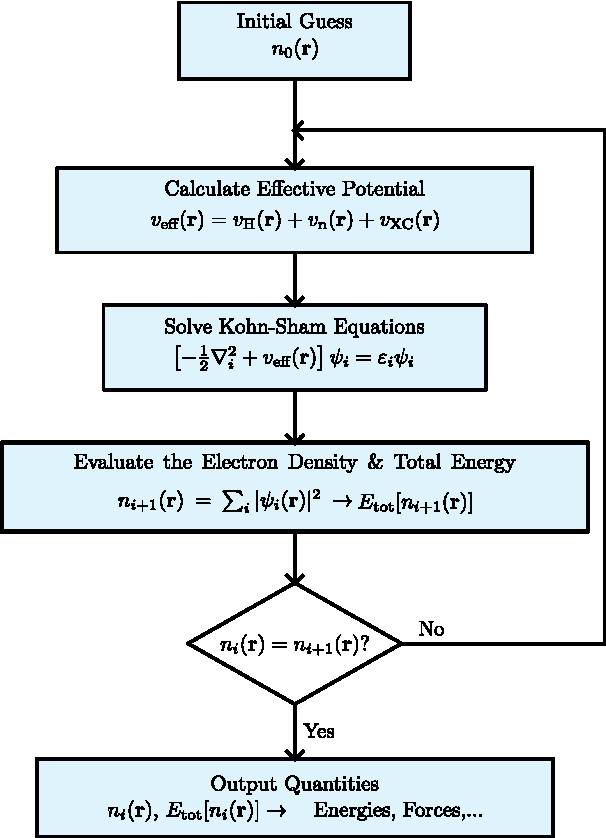
\includegraphics[width=0.6\textwidth]{vasp-workflow.pdf}
    \caption{
        Self-consistent field (SFC) cycle in VASP for DFT calculations adapted from Ref. \cite{sholl2023density}. The entire cycle starts with an initial guess of the electronic density $n_0(\mathbf{r})$, which is then used to calculate the effective potential $v_{\text{eff}}(\mathbf{r})$. Then, the resulting potential is used to solve the Kohn-Sham equations, from which single-electron wavefunctions $\psi_i(\mathbf{r})$ are obtained. Consequently, the new electronic density $n_{i+1}(\mathbf{r})$ is calculated. Should the old and new densities be close enough---up to a predefined threshold---the cycle stops, and the final electronic density is used to calculate the energies, forces, and stress tensor of the system. Otherwise, the cycle repeats itself until convergence is achieved. 
    }
    \label{fig:vasp_workflow}
\end{figure}

\section{VASP Input \& Output Files}
\label{sec:vasp-input-output-files}
The VASP input and output files are essential for our calculations. On the one hand, the input files contain necessary information---such as the initial structure, exchange-correlation functionals, PAW pseudopotentials, k-point grid, and convergence criteria---that guide the different simulations. On the other hand, the output files contain the results of the different simulations, such as the total energy, forces, stress tensor, and the fully relaxed structure.

This section provides an overview of the required input files for VASP calculations, as well as some relevant output files. For a detailed and rather technical description of the files described herein, we refer the reader to the VASP manual \cite{zotero-item-672}.

\subsection{Input Files}
\subsubsection{INCAR}
The \texttt{INCAR} file (see Figure \ref{fig:incar}) defines the computational parameters in VASP and specifies the type of calculation to be performed. Each simulation stage---such as structure optimisation, Density of States (DOS) calculations, AIMD simulations, or MLFF training---is defined by a specific set of INCAR tags. 
\begin{figure}[H]  
	\centering  
	\begin{threeparttable}  
		\caption{Example of an \texttt{INCAR} file used for structure relaxation of  C--S--H. This file specifies the optimisation algorithm, force convergence criteria, exchange-correlation functional (PBEsol) and ionic relaxation parameters. Depending on the type of calculation to be performed, different tags may be added or removed.
        }  
		\label{fig:incar}  
		\resizebox{\textwidth}{!}{  
			\begin{tabular}{>{\columncolor{blue!10}}l>{\columncolor{blue!10}}l>{\columncolor{blue!10}}l>{\columncolor{blue!10}}l>{\columncolor{blue!10}}l>{\columncolor{blue!10}}l>{\columncolor{blue!10}}l>{\columncolor{blue!10}}l>{\columncolor{blue!10}}l>{\columncolor{blue!10}}l>{\columncolor{blue!10}}l>{\columncolor{blue!10}}l>{\columncolor{blue!10}}l>{\columncolor{blue!10}}l>{\columncolor{blue!10}}l>{\columncolor{blue!10}}l>{\columncolor{blue!10}}l>{\columncolor{blue!10}}l>{\columncolor{blue!10}}l}  
				\hline   
				\multicolumn{3}{c}{\cellcolor{blue!10} \textbf{GENERAL}} & & & & & & & & & & & & & & & & \\   
				\textbf{SYSTEM} & \textbf{=  C--S--H} & \textit{\# System name} & & & & & & & & & & & & & & & & \\   
				\textbf{PREC}   & \textbf{= Accurate} & \textit{\# Precision level} & & & & & & & & & & & & & & & & \\   
				\multicolumn{3}{c}{\cellcolor{blue!10} \textbf{ELECTRONIC OPTIMIZATION}} & & & & & & & & & & & & & & & & \\   
				\textbf{ENCUT}  & \textbf{= 800} & \textit{\# Plane-wave cutoff (eV)} & & & & & & & & & & & & & & & & \\   
				\textbf{LREAL}  & \textbf{= Auto} & \textit{\# Real-space projection} & & & & & & & & & & & & & & & & \\   
				\textbf{ISMEAR} & \textbf{= 0} & \textit{\# Smearing method} & & & & & & & & & & & & & & & & \\   
				\textbf{SIGMA}  & \textbf{= 0.05} & \textit{\# Smearing width (eV)} & & & & & & & & & & & & & & & & \\   
				\textbf{ALGO}   & \textbf{= F} & \textit{\# Electronic minimization algorithm} & & & & & & & & & & & & & & & & \\   
				\textbf{AMIX}   & \textbf{= 0.1} & \textit{\# Charge density mixing parameter (damping)} & & & & & & & & & & & & & & & & \\   
				\multicolumn{3}{c}{\cellcolor{blue!10} \textbf{EXCHANGE-CORRELATION / FUNCTIONAL}} & & & & & & & & & & & & & & & & \\   
				\textbf{GGA}    & \textbf{= PS} & \textit{\# PBEsol functional} & & & & & & & & & & & & & & & & \\   
				\textbf{IVDW}   & \textbf{= 11} & \textit{\# DFT-D3(zero) vdW correction} & & & & & & & & & & & & & & & & \\   
				\textbf{LASPH}  & \textbf{= .TRUE.} & \textit{\# Non-spherical contributions} & & & & & & & & & & & & & & & & \\   
				\textbf{LMAXMIX}& \textbf{= 4} & \textit{\# Maximum l for charge mixing} & & & & & & & & & & & & & & & & \\   
				\multicolumn{3}{c}{\cellcolor{blue!10} \textbf{CHARGE \& WAVEFUNCTION}} & & & & & & & & & & & & & & & & \\   
				\textbf{LCHARG} & \textbf{= F} & \textit{\# Do not write CHGCAR} & & & & & & & & & & & & & & & & \\   
				\multicolumn{3}{c}{\cellcolor{blue!10} \textbf{IONIC RELAXATION}} & & & & & & & & & & & & & & & & \\   
				\textbf{NELMIN} & \textbf{= 4} & \textit{\# Minimum SCF steps} & & & & & & & & & & & & & & & & \\   
				\textbf{MAXMIX} & \textbf{= 40} & \textit{\# Maximum mixing steps} & & & & & & & & & & & & & & & & \\   
				\textbf{IBRION} & \textbf{= 2} & \textit{\# Ionic relaxation algorithm} & & & & & & & & & & & & & & & & \\   
				\textbf{ISIF}   & \textbf{= 3} & \textit{\# Relax ions + cell shape + volume} & & & & & & & & & & & & & & & & \\   
				\textbf{NSW}    & \textbf{= 700} & \textit{\# Maximum ionic steps} & & & & & & & & & & & & & & & & \\   
				\textbf{EDIFFG} & \textbf{= -0.02} & \textit{\# Convergence criterion (eV/\AA)} & & & & & & & & & & & & & & & & \\   
				\textbf{ADDGRID}& \textbf{= T} & \textit{\# Additional grid for accuracy} & & & & & & & & & & & & & & & & \\   
				\hline  
			\end{tabular}  
		}  
	\end{threeparttable}  
\end{figure}
These parameters control convergence thresholds, exchange-correlation functionals, long-range corrections, ensemble choices, and other simulation parameters. If not specified by the user, VASP uses default values. Nonetheless, for reliable and reproducible results, the main parameters must be tailored to the system and the type of calculation.


\subsubsection{POSCAR}
The \texttt{POSCAR} (see Figure \ref{fig:csh_poscar}) file provides the actual structure to be studied. It is subdivided into several sections, each one providing specific information about the system.
\begin{figure}[H]
\resizebox{\textwidth}{!}{
\begin{tabular}{>{\columncolor{blue!10}}c>{\columncolor{blue!10}}c>{\columncolor{blue!10}}c
>{\columncolor{blue!10}}l>{\columncolor{blue!10}}l>{\columncolor{blue!10}}l>{\columncolor{blue!10}}l
>{\columncolor{blue!10}}l>{\columncolor{blue!10}}l>{\columncolor{blue!10}}l>{\columncolor{blue!10}}l
>{\columncolor{blue!10}}l>{\columncolor{blue!10}}l>{\columncolor{blue!10}}l>{\columncolor{blue!10}}l
>{\columncolor{blue!10}}l>{\columncolor{blue!10}}l>{\columncolor{blue!10}}l>{\columncolor{blue!10}}l
>{\columncolor{blue!10}}l>{\columncolor{blue!10}}l>{\columncolor{blue!10}}l>{\columncolor{blue!10}}l
>{\columncolor{blue!10}}l>{\columncolor{blue!10}}l}
\hline
\multicolumn{3}{l}{\cellcolor{blue!10} \textbf{Ca Si O H}} & & & & & & & & & & & & & & & & & & & & & & \\
\multicolumn{3}{l}{\cellcolor{blue!10}1.0} & & & & & & & & & & & & & & & & & & & & & & \\
13.18335946 & 0.18445997 & 0.00755401 & & & & & & & & & & & & & & & & & & & & & & \\
-16.45244030 & 24.21622147 & -0.00875423 & & & & & & & & & & & & & & & & & & & & & & \\
1.20664987 & -0.82375620 & 23.18729854 & & & & & & & & & & & & & & & & & & & & & & \\
\multicolumn{3}{l}{\cellcolor{blue!10} \textbf{Ca Si O H}} & & & & & & & & & & & & & & & & & & & & & & \\
\multicolumn{3}{l}{\cellcolor{blue!10}99 60 323 208} & & & & & & & & & & & & & & & & & & & & & & \\
\multicolumn{3}{l}{\cellcolor{blue!10}Direct} & & & & & & & & & & & & & & & & & & & & & & \\
0.38821570 & 0.10613519 & 0.29312228 & & & & & & & & & & & & & & & & & & & & & & \\
0.37259751 & 0.56538816 & 0.26881558 & & & & & & & & & & & & & & & & & & & & & & \\
0.37469040 & 0.31600944 & 0.23882914 & & & & & & & & & & & & & & & & & & & & & & \\
0.35542617 & 0.78384113 & 0.38748504 & & & & & & & & & & & & & & & & & & & & & & \\
0.91347068 & 0.11233954 & 0.31634176 & & & & & & & & & & & & & & & & & & & & & & \\
0.90355777 & 0.57838562 & 0.23567872 & & & & & & & & & & & & & & & & & & & & & & \\
0.87836092 & 0.32109531 & 0.25338100 & & & & & & & & & & & & & & & & & & & & & & \\
0.84529168 & 0.81264469 & 0.29236748 & & & & & & & & & & & & & & & & & & & & & & \\
0.11769176 & 0.02588977 & 0.65372010 & & & & & & & & & & & & & & & & & & & & & & \\
\hline
\end{tabular}
}
\caption{Unit cell structure in fractional coordinates for the C--S--H (Calcium Silicate Hydrates) system. The lattice vectors, atomic species (99 Ca, 60 Si, 323 O, 208 H), and the first 9 atomic positions are shown. All coordinates are expressed in direct (fractional) form.}
\label{fig:csh_poscar}
\end{figure}
The first line contains a comment specifying the name of the system or a brief description of it. Lines 2-4 provide the scaling factor and the corresponding lattice vectors. The actual lattice vectors are obtained by multiplying the scaling factor (line 2) by the numbers in lines 3-5. Lines 6-7 specify the atomic species as well as the number of ions of each species. Finally, lines 9-onwards provide the ionic positions in angstroms. 

\subsubsection{KPOINTS}
Defining the k-point grid is an essential and one of the first steps when performing DFT calculations, as the accuracy and convergence of the results depend on it. Figure \ref{kpoints} illustrates the \texttt{KPOINTS} file used in this work. The specified mesh is a $1\times 1\times 1$ Gamma-centered grid, obtained after a convergence test. 
\begin{figure}[H]
\resizebox{\textwidth}{!}{
	\begin{tabular}{>{\columncolor{blue!10}}c>{\columncolor{blue!10}}l>{\columncolor{blue!10}}l>{\columncolor{blue!10}}l>{\columncolor{blue!10}}l>{\columncolor{blue!10}}l>{\columncolor{blue!10}}l>{\columncolor{blue!10}}l>{\columncolor{blue!10}}l>{\columncolor{blue!10}}l>{\columncolor{blue!10}}l>{\columncolor{blue!10}}l>{\columncolor{blue!10}}l>{\columncolor{blue!10}}l>{\columncolor{blue!10}}l>{\columncolor{blue!10}}l>{\columncolor{blue!10}}l>{\columncolor{blue!10}}l>{\columncolor{blue!10}}l>{\columncolor{blue!10}}l>{\columncolor{blue!10}}l>{\columncolor{blue!10}}l>{\columncolor{blue!10}}l>{\columncolor{blue!10}}l>{\columncolor{blue!10}}l>{\columncolor{blue!10}}l>{\columncolor{blue!10}}l>{\columncolor{blue!10}}l>{\columncolor{blue!10}}l>{\columncolor{blue!10}}l>{\columncolor{blue!10}}l>{\columncolor{blue!10}}l>{\columncolor{blue!10}}l>{\columncolor{blue!10}}l>{\columncolor{blue!10}}l>{\columncolor{blue!10}}l>{\columncolor{blue!10}}l} \hline
		\multicolumn{1}{l}{\cellcolor{blue!10} \textbf{ C--S--H kpoints}} & & & & & & & & & & & & & & & & & & & & & & & & & & & & & & & & & & & &\\ 
		\multicolumn{1}{l}{\cellcolor{blue!10}0}& & & & & & & & & & & & & & & & & & & & & & & & & & & & & & & & & & & &\\
		\multicolumn{1}{l}{\cellcolor{blue!10} \textbf{Gamma}}& & & & & & & & & & & & & & & & & & & & & & & & & & & & & & & & & & & &\\ 
		1 1 1& & & & & & & & & & & & & & & & & & & & & & & & & & & & & & & & & & & & \\
		0 0 0& & & & & & & & & & & & & & & & & & & & & & & & & & & & & & & & & & & & \\  \hline
	\end{tabular}
 }
	\centering
	\caption{ C--S--H k-point grid centered at the Gamma point. The values "1 1 1" define the grid dimensions in the $x$, $y$, and $z$ directions. For large systems, a Gamma-centered grid is enough to achieve convergence.}
	\label{kpoints}
\end{figure}

\subsubsection{POTCAR}
The \texttt{POTCAR} file contains the PAW pseudopotentials for each atomic species in the system. As such, it defines how valence electrons interact with the atomic cores. It is constructed by concatenating the individual POTCAR files for each species into a single file. In our work,  we employed the following PAW pseudopotentials from the PAW\_PBE library:
\begin{itemize}
    \item Ca: Ca\_pv ([Ar] 4s$^2$)
    \item Si: Si ([Ne] 3s$^2$ 3p$^2$)
    \item O: O ([He] 2s$^2$ 2p$^4$)
    \item H: H (1s$^1$)
\end{itemize}

\subsection{Output Files}
These are the primary output files generated upon finishing an FP calculation in VASP. They provide core information regarding the performance of the calculations, documenting the simulation and providing the basis for further analysis.
\subsubsection{OUTCAR}
The \texttt{OUTCAR} file is a comprehensive output file that contains detailed information about the VASP calculation. It includes a summary of the input parameters, the evolution of the SCF cycle, the total energy, forces on the atoms, and the stress tensor.
\subsubsection{CONTCAR}
The \texttt{CONTCAR} file records the final atomic positions and lattice vectors after a structure relaxation or optimisation. Additionally, this file may also contain atomic velocities and predictor-corrector information if it was written during an AIMD simulation. It has a compatible format with the \texttt{POSCAR} file, making it possible to use it as an input structure for subsequent calculations.

\subsubsection{DOSCAR}
The \texttt{DOSCAR} file stores the Density of States (DOS) and integrated DOS, expressed in states/eV and cumulative number of states, respectively. This data is beneficial for analysing the electronic properties of the system, and understanding features such as the band gap and the distribution of states across the valence and conduction bands. 
\subsubsection{OSZICAR}
The \texttt{OSZICAR} file records a summary of the electronic and ionic iterations during a DFT calculation. It allows the user to monitor the progress of the SCF cycle convergence, visualise changes in the total energy, and follow the evolution of the ionic relaxation process. 
\subsubsection{ML\_ABN}
The \texttt{ML\_ABN} file contains the training dataset collected during an on-the-fly MLFF training process. As previously described, the MLFF is trained together with an AIMD simulation, where atomic configurations are sampled. Representative configurations are then written to this file, which can be reused to continue the training by renaming it to a \texttt{ML\_AB} file.

\subsubsection{ML\_FFN}
The \texttt{ML\_FFN} file is a binary file that stores the trained machine learning force field (MLFF) model at the end of the training phase. It contains the model parameters, such as weights and hyperparameters, that define the MLFF. The model can be used for prediction or further refinement by renaming it to an \texttt{ML\_FF} file.


\section{Strucure Relaxation}
\label{sec:structure-relaxation}
Relaxing the  C--S--H structure is a crucial step towards obtaining equilibrium properties of this material. This process involves minimising both the forces on atoms and the total energy of the system, leading to a stable configuration. In this work, we performed structure relaxation in two stages: an initial relaxation was conducted using DFTB+, which provided a good starting point for VASP and reduced the computational cost of the full structure relaxation. The second stage consists of a full structure relaxation using VASP. Here we outline both stages of the structure relaxation process.

\subsection{Initial Relaxation with DFTB+}
Given the large size of the  C--S--H structure, it was necessary to perform a preliminary relaxation using the GFN1-xTB method implemented in DFTB+. For this step, we first conducted a k-point convergence test. We then plugged this value into the relaxation script in order to run the structure relaxation. This trick allows us to take our structure closer to its equilibrium configuration, without spending too much time and computational power to do so. This approach is valid because we are not using the final structure as our actual optimised structure, but rather as a means to reduce the computation time required for full structure relaxation in VASP.  

\subsection{Full Structure Relaxation with VASP}
After the rough approximation provided by DFTB+, a full structure relaxation is performed using VASP. To achieve this, we first perform a cut-off energy convergence test, followed by a k-point convergence test. Thereafter, we define the k-point mesh in the \texttt{KPOINTS} file, and the cut-off energy in the \texttt{INCAR} file, where we also specified the PBEsol functional and a force convergence criteria of 0.02 eV/\AA. Once the structure has been fully relaxed, it is used to study the Density of States (DOS) and to train the machine learning force field.

\section{Machine Learning Force Field Generation}
\label{sec:mlff-generation}
This stage is subdivided into three main phases: training, refinement, and testing. In this section, we describe each one of them in detail.
\subsection{Training}
As previously discussed, the MLFF is generated on-the-fly during an AIMD simulation. To begin, we use the \texttt{CONTCAR} file, which contains our relaxed structure, as the input \texttt{POSCAR} file for this step. In the \texttt{INCAR} file some parameters need to be set: \texttt{IBRION=0}, indicates VASP to switch to an AIMD simulation; \texttt{NSW=50000} indicates the number of ionic steps; \texttt{POTIM=2.0} is the MD time step in fs; \texttt{MDALGO=3} tells VASP to use the Langevin thermostat; \texttt{TEBEG=400} sets the temperature (in K) at which the simulation is performed, and \texttt{ISIF=3} allows for positions, cell shape and volume to be~updated. 

Finally, \texttt{ML\_LMLFF=T} and \texttt{ML\_ISTART=0} tags govern the MLFF training process. The former enables the use of machine learning force fields, and the latter tells VASP to generate a new MLFF from scratch. Although the parameters described herein are the most important, additional tags may need to be set depending on the performance of the training phase.

\subsection{Refinement}
The refinement phase allows for improvements to be made in the generated MLFF by tuning the hyperparameters in the model. To this end, we first generate a set of 50000 structures using the force field, from which we uniformly sample 50 configurations. Then we compute the total energy, forces and stress tensor for each one of them in two separate runs. The first run utilises first principles, whereas the second run is performed using the MLFF model. The corresponding data is then postprocessed and the errors between DFT and MLFF results are evaluated using configuration-wise Root Mean Square Error (RMSE) defined as follows:
\begin{subequations}
    \label{eq:rmse_per_conf}
    \begin{align}
        \label{eq:energy_error}
        E^i_{\text{error}} &= \frac{E_i^{\text{DFT}} - E_i^{\text{MLFF}}}{\text{N}_{a}} \\
        \label{eq:force_error}
        F^i_{\text{RMSE}} &= \sqrt{\frac{1}{3\text{N}_{a}}\sum_{j=1}^{\text{N}_{a}}\sum_{k=1}^{3} \left(\mathbf{F}_{ijk}^{\text{DFT}} - \mathbf{F}_{ijk}^{\text{MLFF}}\right)^2} \\
        \label{eq:stress_error}
        S^i_{\text{RMSE}} &= \sqrt{\frac{1}{6} \sum_{\alpha=1}^{3}\sum_{\beta=1}^{3} \left(\sigma_{i\alpha\beta}^{\text{DFT}} - \sigma_{i\alpha\beta}^{\text{MLFF}}\right)^2}
    \end{align}
\end{subequations}
where $i$ indicates the configuration index, $\text{N}_a$ is the number of atoms in the system, $j$ is the atom index, $k$ corresponds to the Cartesian components of the forces, and $\alpha$, $\beta$ are the Cartesian indices of the stress tensor. Note that the energy error does not correspond to a RMSE, but rather to a per-atom energy error. Likewise, global RMSE values for the entire set of configurations are computed as follows:
\begin{subequations}
    \label{eq:rmse_global}
    \begin{align}
        \label{eq:rmse_e}
        E_{\text{RMSE}} &= \sqrt{\frac{1}{\text{N}_s}\sum_{i=1}^{\text{N}_s} \left(E_i^{\text{DFT}} - E_i^{\text{MLFF}}\right)^2} \\
        \label{eq:rmse_f}
        F_{\text{RMSE}} &= \sqrt{\frac{1}{\text{N}_{s}} \sum_{i=1}^{\text{N}_{s}} \left(F^i_{\text{RMSE}} \right)^2} \\
        \label{eq:rmse_s}
        S_{\text{RMSE}} &= \sqrt{\frac{1}{\text{N}_s} \sum_{i=1}^{N_s} \left(S^i_{\text{RMSE}} \right)^2}
    \end{align}
\end{subequations}
where $\text{N}_s$ is the total number of sampled configurations. These results are significant as they provide the means to evaluate the performance of our force field.

Afterwards, we conduct a hyperparameter optimisation in order to improve the performance of the force field. It is noteworthy that VASP provides various hyperparameters that we can optimise; nevertheless, in this work, only two hyperparameters were considered---the two and three-body descriptors---as they directly affect the accuracy of the force field. In this regard, we set \texttt{ML\_MODE=refit} and \texttt{ML\_RCUT1=\#} in the \texttt{INCAR} file. The latter parameter corresponds to the radial descriptor (given in \AA), and is to be modified accordingly to a reasonable range. Thereafter, we use the resulting MLFF file to evaluate the performance of the refitted force field for the given \texttt{RCUT1}. We achieve this by setting \texttt{IBRION=-1} and \texttt{ML\_MODE=run} in the \texttt{INCAR} file. This calculation will return the RMSE for energies, forces, and the stress tensor as a function of the descriptor. The same process is then applied to the angular descriptor \texttt{RCUT2}, and the optimal hyperparameters are chosen to minimise the errors. 

\subsection{Testing}
Following the refinement process, we can utilise the MLFF model to conduct various simulations, including AIMD simulations, structure relaxation, and other DFT calculations. In this work, we used the generated force field to compute the equation of state (EOS) of  C--S--H. Additionally, we also performed a simulated annealing process to obtain a more stable structure and computed its corresponding EOS as well. Finally, various MD simulations were conducted at temperatures of 200, 250, 300, 350, and 400 K to study the transferability of the force field as well as the expansion coefficient of  C--S--H.
